\chapter{Evaluation}
\label{cha:evaluation}

We found that it is possible to build our application for the HoloLens that works as intended but we still had to overcome a few problems and faced some challenges. These are the difficulties we had to deal with:

\begin{description}[align=left]
	\item [Wrong orientation matrix] 
	This problem affected us right in the beginning. For getting all our bricks at the right place, we have to transform all the points that we read from the input. For that, every brick file that gets added per step has its own transformation matrix defined. We now have to transform all the points inside of the new file to have the bricks where the file wants them to be. The error we made was that we also have to transform the new transformation matrices inside of the file and not just the points. The result was that the points and triangles in the first layer of files would be in the right position but any others would be wrong.
	
	\item [Color] 
	To get the color of the models right was difficult. The .ldr file defines the color at the beginning of every file, line, triangle or quad with help of a single integer. This number then has to be looked up to find the actual color. Some of the numbers also define other behaviors, like to take the same color as the brick one layer above, or the complementary color. \newline 
	The fist approach was to define vertex colors, to give every point in the .obj file a RGB value. That works great if we work with programs that can interpret and parse the vertex color like MeshLab~\cite{meshlab}, which we used to test the output of the Python script. The problem emerged when we started with the second step and tried to load our objects in Unity to build our application. The Unity .obj parser does not understand vertex colors, so to interpret them we would have to use a custom shader. \newline 
	The other option we have is to use a material library file (.mtl) and write all the colors/materials in there, instead of defining them per vertex. Now we just have to write a separate file with all the colors and define which ones we are using in front of the triangle lines in the .obj file. With that, Unity can create the materials itself to add them to the models.
	
	\item [Shading]
	The way the shader, that is added to a loaded .obj mesh in Unity, defines the outside of a face, is to take the direction of the normal of it and then just colors this side. The other side of it is see-trough. The problem we have is that in the preprocessing script we have no normals and therefore also do not know which side is outside or inside. That means we can not write them in the .obj files. \newline 
	Unity now takes the points in the order they are given in the file to calculate the normal of each face. That does not always work as we can see in Figure~\ref{fig:wrong_shaded}. To solve that we can either write our own shader that colors both sides of the faces, or we take the easier way and define every face twice. We switch the order of the points that they are defined by and so effectively switch the normal. The outcome can be seen in Figure~\ref{fig:right_shaded}. Even though we have a little overhead now (every polygon is defined twice), it saved us time with writing a shader and from possible problems that we could have gotten with shading both sides of the faces.
	
	\begin{figure}[!ht]
		\captionsetup{justification=centering}
		\centering
		\subfloat[{Shading of front side of polygones.}]{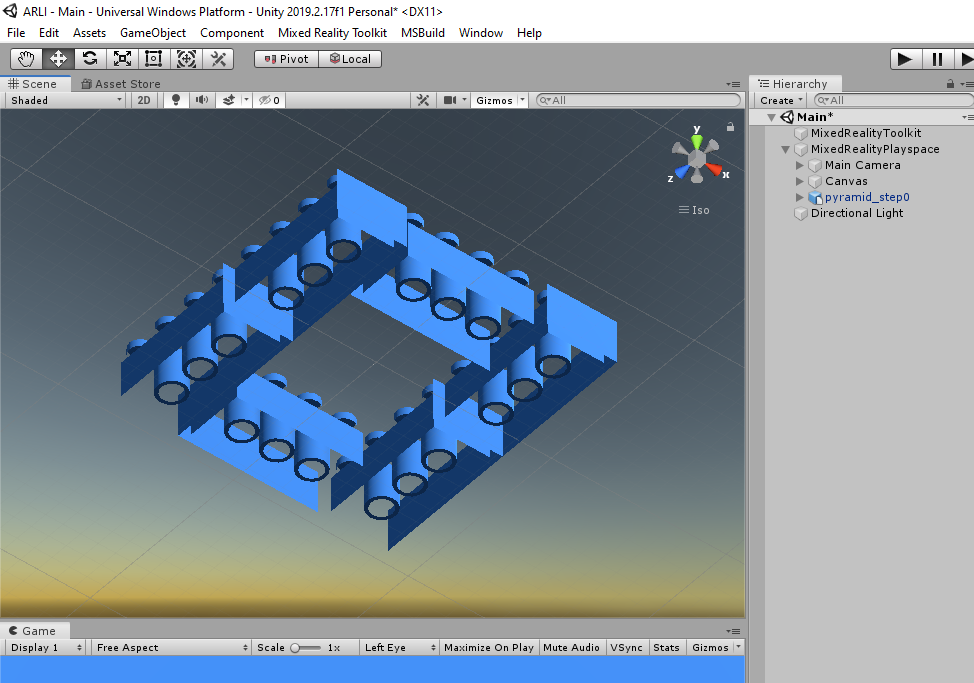
\includegraphics[width=0.47\textwidth]{media/wrong_shaded.png}\label{fig:wrong_shaded}}
		\hfill
		\subfloat[{Shading of both polygon sides.}]{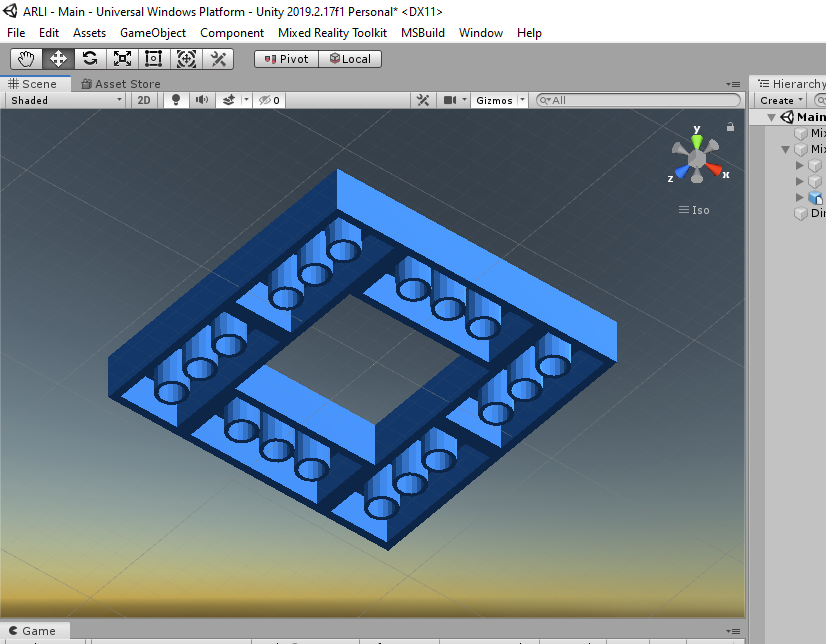
\includegraphics[width=0.47\textwidth]{media/right_shaded.png}\label{fig:right_shaded}}
		\hfill
		\caption{Shading with one sided vs. double sided polygons.}
		\label{fig:shading.}
	\end{figure}

	\newpage
	
	\item [Lighting]
	To make the the model clearly visible we decided to add an extra directional light to the scene. We could also just use ambient lighting but this was just not bright enough. We also want to take advantage of shadows to bring out the features of the models.\newline To always have the light from the front and do not have a darker side, the added light is attached to the camera. In this way the light always comes from the users head. 
	
	\item [Lines]
	Another big problem we have with the .obj format is that the Unity parser does not know what to do with the lines defined between two vertices. All the models just have an uniform color and we can not distinguish between different bricks. \newline 
	One fix for that would be using texture mapping but since we do not have texture pictures and do not want to create them for every single brick we are using, this is not optimal. A possible solution that we were trying, is to write all our lines to a separate file that we were parsing manually. In our C\# script that we are using to load the current model, we are reading the lines file, a simple plain text file, and create and add all the lines. Unfortunately, that is a large overhead, even with a simple model we do not get more than 10 frames per second like we can see in Figure~\ref{fig:lines_fps}. Since there is not really any other good way, the best is to not add lines. With shadows turned on we can still recognize most of the parts and we even get decent performance as seen in Figure~\ref{fig:without_lines_fps}.
	
	\begin{figure}[!ht]
		\captionsetup{justification=centering}
		\centering
		\subfloat[{Added lines with bad performance.}]{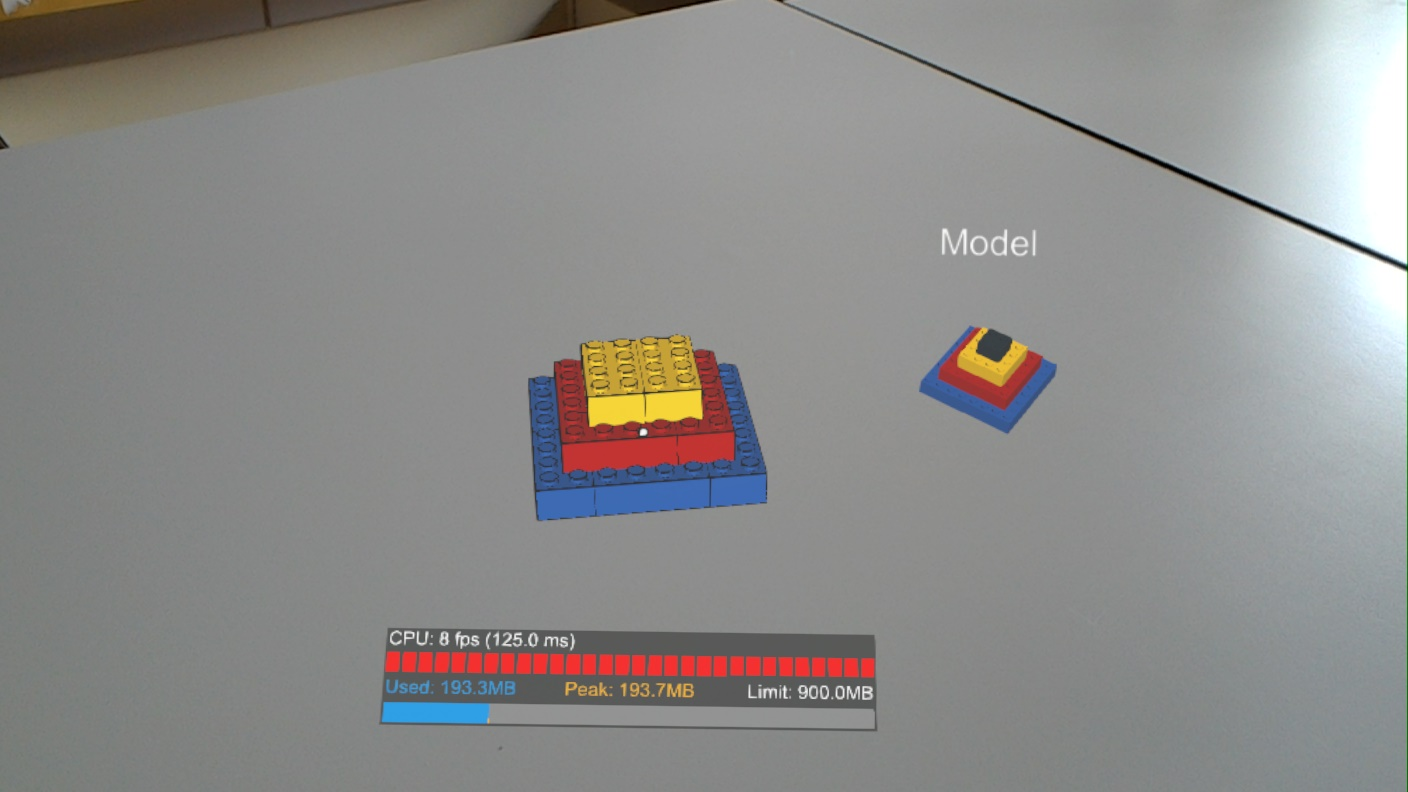
\includegraphics[width=0.47\textwidth]{media/bad_performance.jpg}\label{fig:lines_fps}}
		\hfill
		\subfloat[{Decent performance without lines.}]{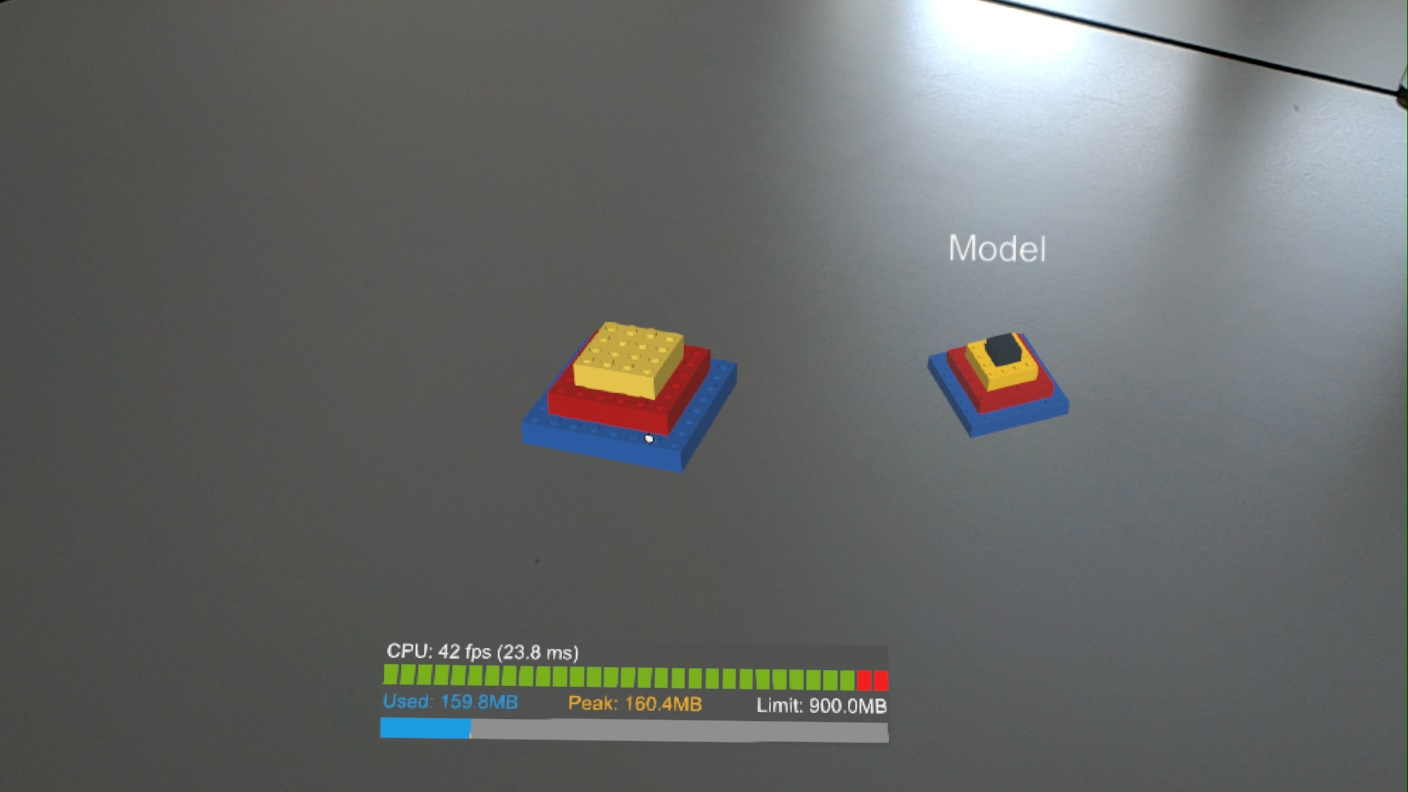
\includegraphics[width=0.47\textwidth]{media/good_performance.jpg}\label{fig:without_lines_fps}}
		\hfill
		\caption{Performance difference when adding lines to the model.}
		\label{fig:lines_performance}
	\end{figure}

	\newpage
		
	\item [Scaling of preview]
	Scaling of the model is normally not a problem since the input files have the measurements in real life and the model that gets shown on the HoloLens can be scaled by the user. The only real issue we have is the preview in the upper right corner. It has a fixed size and moves with the user so it will always stay at the same place. If we now have a bigger figure, like for example a whole building that is 30 centimeters tall, it can happen that parts of it will be out of the field of view, in case it is not scaled down as seen in Figure~\ref{fig:preview_scaling} (the actual field of view when wearing the HoloLens is smaller as on the figures). Other, smaller models will be, when scaled down, too small to see. The best approach we have is to define a bounding box around the model and scale the model according to that.
	
	\begin{figure}[!ht]
		\captionsetup{justification=centering}
		\centering
		\subfloat[{Good scaling with a small enough model.}]{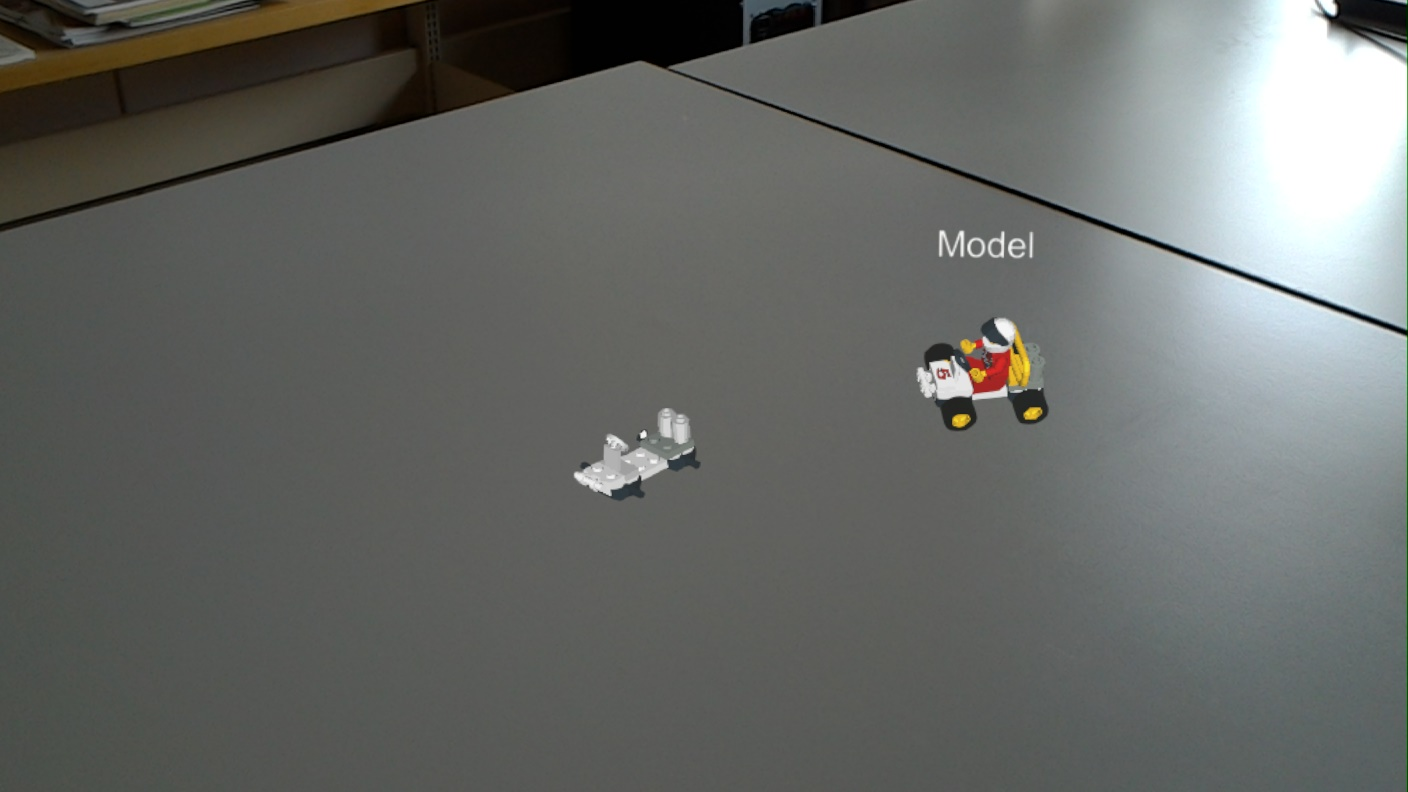
\includegraphics[width=0.47\textwidth]{media/preview_good.jpg}\label{fig:smp}}
		\hfill
		\subfloat[{Bad scaling with a too big model.}]{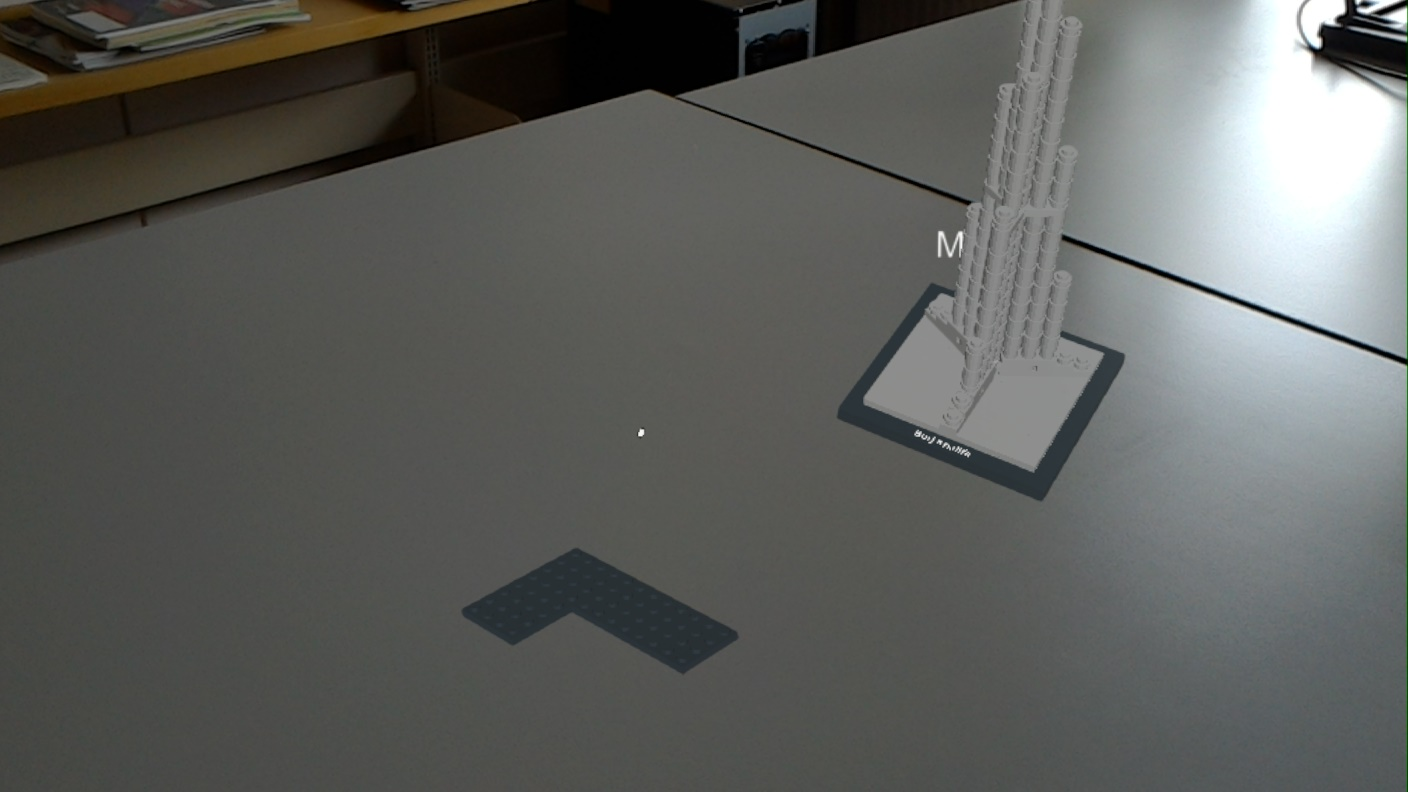
\includegraphics[width=0.47\textwidth]{media/preview_big.jpg}\label{fig:smb}}
		\hfill
		\caption{Preview scaling of two different sized models.}
		\label{fig:preview_scaling}
	\end{figure}
	
	\item [Parsing]
	We had serious problems on multiple occasions, when we were trying to parse the files, simply because of the fact that the model description files we are using are from the official model repository~\cite{omr}. Even though the files there should be all the same and follow the specification from the LDraw website, they still slightly differ. The fact that not every model description has defined steps, or some just have them in the sub-files, makes it hard to find out all individual steps and also which bricks are used when.
	
	\item[Model Picker Billboard] 
	On the start screen, where we pick our model, we have a canvas with user interface (UI) elements on it. With our first design, once the user looked away from it, the canvas with the text and the drop down box stayed where it was. When returning back to it from one instruction, it was where the app first booted up. But we want it to behave more like a billboard that follows the users gaze. For that, we had to add a Solver Handler script that tracks the head movement and Radial View script that defines the parameters like max and min view degrees and min and max distance of the canvas, pictured in Figure~\ref{fig:tagalong}.
	
	\begin{figure}[!ht]
		\captionsetup{justification=centering}
		\centering
		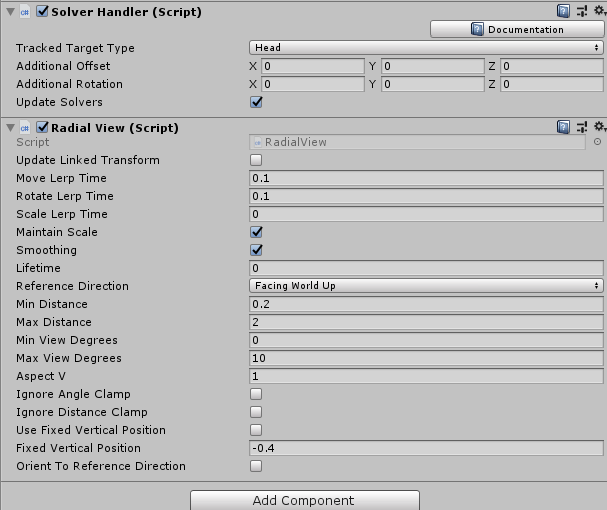
\includegraphics[width=0.8\textwidth]{media/tagalong.png}
		\hfill
		\caption{Scripts added to the model picker to make it move along with the user.}
		\label{fig:tagalong}
	\end{figure} 

	\item[Runtime model adding]
	Even though the idea in the beginning was to implement runtime adding from new models, it turned out to be harder and more complicated. At first we fixed the model to the app, depending on the chosen model in the beginning, we loaded a prepared scene. That worked but was not optimal since we want the models loaded at runtime. \newline 
	The second approach was to put every model we have in the resources folder in the application, so that the model files would be part of the build and can be loaded at execution. The problem here is that all models and files for them have to be written before building the app and once built we can not add any new LEGO builds. Every model .ldr file has to be preprocessed with the Python script and the created files saved in the build directories before we can build our application for the HoloLens. \newline 
	Another way to load resources at time of execution of an already built app in Unity, is to use asset bundles\footnote{\url{https://docs.unity3d.com/Manual/AssetBundlesIntro.html}}. These can be loaded from everywhere on the file system where the app runs, or even better, from a web server. The problem is the building of these packages. While before Unity 5 it was possible to build them via a C\# script, with Unity 5 it changed and is now only possible in the editor. \newline 
	For the user that means, for creating asset packages with newly preprocessed models, it is necessary to open Unity and create the bundles there and then copy it to the HoloLens. That is almost the same amount of work as if we just recompile the Unity app and deploy it to the HoloLens again. In the end we implemented a mix form, we are building asset bundles ``per hand'' and put them in the streaming asset folder. Files from there get copied to the device and will be at the same location where we could store assets from web requests (more on that in Chapter~\ref{sec:changes}). From there we can load all our resources.
	
\end{description}

\section{Conclusion}

In conclusion we can say that even though we had some problems along the way, we were able to fix them in a reasonable way to make our application work and fulfill the requirements. We came up with a working prototype app that runs on the HoloLens but we also found the limitations of our implementation. We saw that the color/material loading in Unity still has problems, that the insertion of lines is, in terms of frames per second, not tolerable and that large models do not work with reasonable performance.	